%
\documentclass[12pt]{ociamthesis}
\usepackage{tikz}
\newcommand{\id}{\mathrm{id}}
\begin{document}

\begin{equation*}
\begin{aligned}
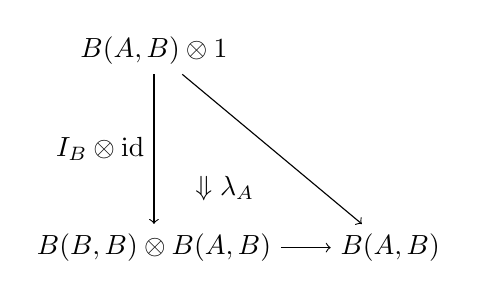
\begin{tikzpicture}[yscale=2.5, xscale=3]
\node (A) at (0,1){${\cat B}(A,B) \otimes 1$};
\node (B) at (1,0) {${\cat B}(A,B)$};
\node (D) at (0,0) {${\cat B}(B,B) \otimes {\cat B}(A,B)$};
\node (C) at (.3,.3){$\Downarrow \lambda_{A}$};
\draw[->] (A) to node[above]{$\iso$} (B);
\draw[->] (D) to node[below]{$\comp$} (B);
\draw[->] (A) to node[left]{$  I_B \otimes \id$} (D);
\end{tikzpicture}
\hspace{1cm}
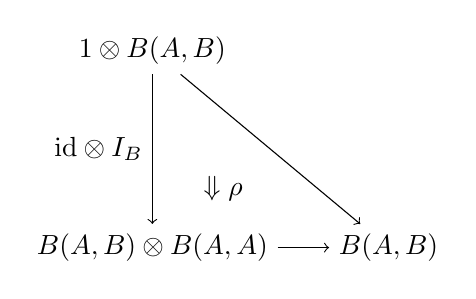
\begin{tikzpicture}[yscale=2.5, xscale=3]
\node (A) at (0,1){$1 \otimes {\cat B}(A,B)$};
\node (B) at (1,0) {${\cat B}(A,B)$};
\node (D) at (0,0) {${\cat B}(A,B) \otimes {\cat B}(A,A)$};
\node (C) at (.3,.3){$\Downarrow\rho$};
\draw[->] (A) to node[above]{$\iso$} (B);
\draw[->] (D) to node[below]{$\comp$} (B);
\draw[->] (A) to node[left]{$\id \otimes I_B$} (D);
\end{tikzpicture}
\end{aligned}
\end{equation*}
\end{document} 
